\begin{tikzpicture}
	\node[anchor=center] {
		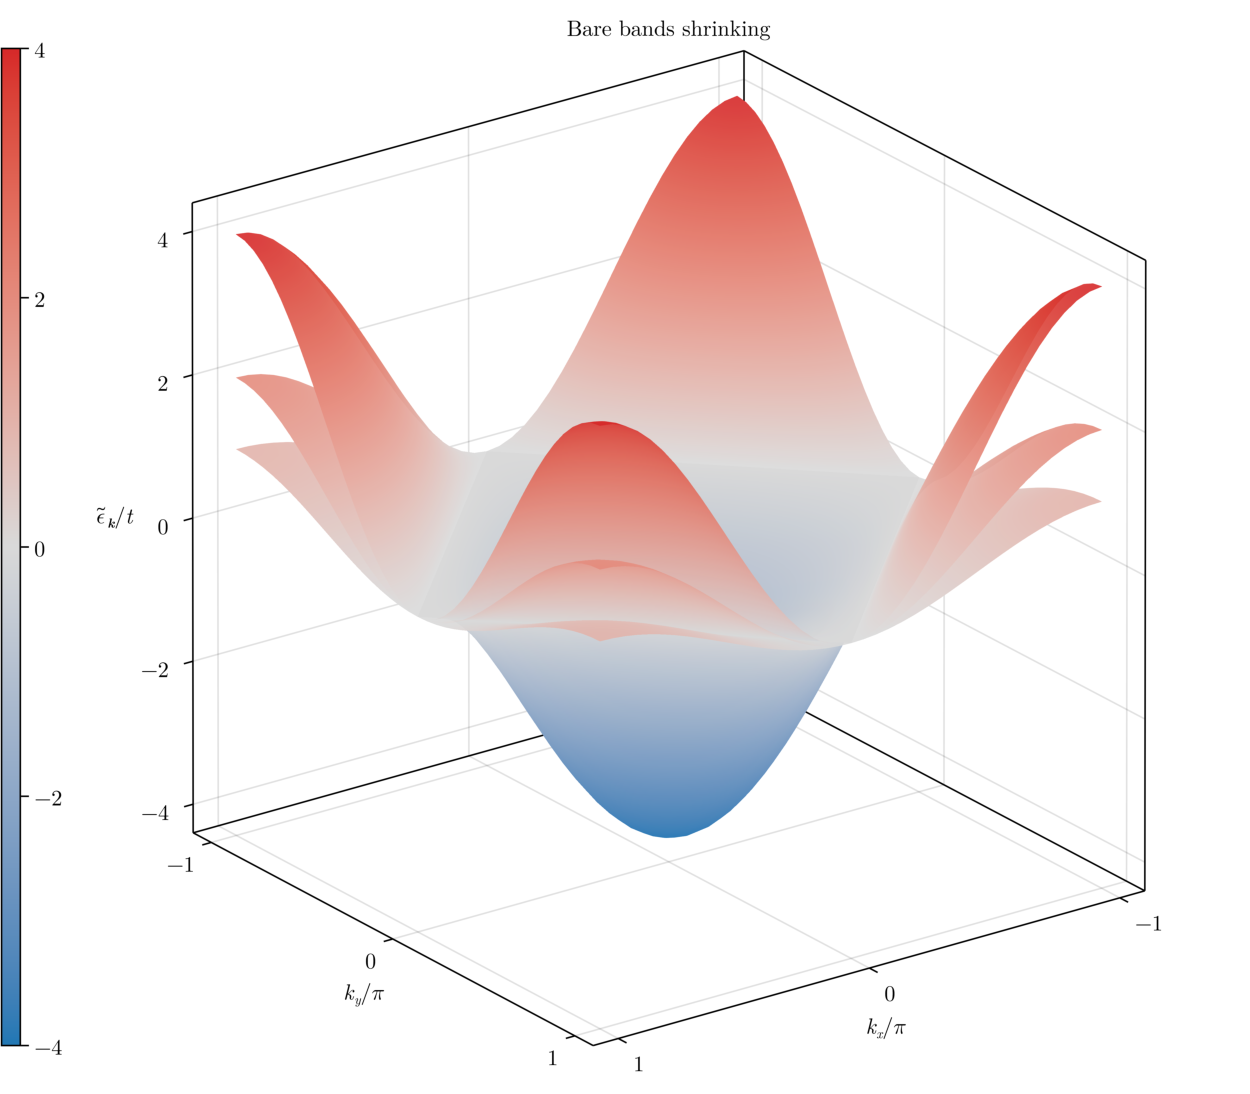
\includegraphics[width=0.6\linewidth]{../Project/src/labs/normal-bands-shrinking/normal-bands-shrinking.pdf}
	};
	
	\draw[color=black] (3.5,1.88) -- ++ (1.5,0)
		node[anchor=west,xshift=0.2em] 
			{$\tilde{t}^{(s^*)}=t$};
			
	\draw[color=black] (3.5,0.84) -- ++ (1.5,0)
		node[anchor=west,xshift=0.2em] 
			{$\tilde{t}^{(s^*)}=t/2$};

	\draw[color=black] (3.5,0.32) -- ++ (1.5,0)
		node[anchor=west,xshift=0.2em] 
			{$\tilde{t}^{(s^*)}=t/4$};
			
\end{tikzpicture}